%! TEX program = xelatex
%        File: slides.tex
%     Created: Sab Apr 22 12:00 pm 2017 C
% Last Change: Sab Apr 22 12:00 pm 2017 C
%
% {{{ PREAMBLE
\documentclass[10pt]{beamer}
%\PassOptionsToPackage{bookmarks=false, hidelinks}{hyperref}
\usepackage[english]{babel}
\usepackage{subfigure}
\usepackage[T1]{fontenc}
\usepackage{microtype}
\usepackage{booktabs}
\usepackage{multirow}
\usepackage{tikz}
\usepackage[compat=1.1.0]{tikz-feynman}
\usepackage{pgfplots}
\usetikzlibrary{arrows,shapes,backgrounds}
\usetikzlibrary{pgfplots.groupplots}
\usepgfplotslibrary{fillbetween}
\usepgfplotslibrary{external}
\tikzexternalize
\tikzsetexternalprefix{log/}
\usepackage{adjustbox}
%\usepackage[mode=buildnew]{standalone}
\usepackage[absolute,overlay]{textpos}
\usepackage{xcolor}
\usepackage[version=4]{mhchem}
%\usepackage{tcolorbox}
\usepackage[most]{tcolorbox}
\newtcolorbox{simpleblock}{
%  enhanced,  % does not work with tikz/external
  boxsep=0.25ex,
%  arc=1.25ex,
  arc=0ex,
  opacityframe=.6,
  opacityback=.6,
  colback=bg!80!fg,
  colframe=white,
  boxrule=0pt,
}
%\usepackage{listings}
%\lstset{language=C++}
%\lstset{
%		basicstyle=\small\ttfamily,
%		keywordstyle=\color{blue}\bfseries,
%		commentstyle=\color{darkgray},
%		stringstyle=\color{orange}
%		}
% define
\usepackage{amsmath}
\renewcommand{\epsilon}{\varepsilon}
\renewcommand{\theta}{\vartheta}
\renewcommand{\rho}{\varrho}
\renewcommand{\phi}{\varphi}
\newcommand{\aof}{\mathring{a}_\text{of}^{(3)}}
\newcommand{\nbb}{\nu\beta\beta}
\newcommand{\Tnu}{T_{1/2}^{2\nu}}
\newcommand{\gerda}{\textsc{Gerda}}
%\includeonlyframes{9}
% metropolis theme options
\usetheme[numbering=fraction]{metropolis}
\usepackage{appendixnumberbeamer}
\setbeamertemplate{frame footer}{Luigi Pertoldi --- \textsc{Tesi di Laurea Magistrale} --- 18/07/2017}
%\setbeamercolor{background canvas}{bg=white}
\setbeamercovered{dynamic}
\title{Ricerca di violazioni delle simmetrie di Lorentz e CPT nel decadimento doppio-beta \texorpdfstring{$2\nbb$}{2nbb} utilizzando i dati dell'esperimento {\gerda}}
\titlegraphic{\vspace{4.8cm}\begin{flushright}
\includegraphics[width=1.8cm]{img/infn-logo.pdf}\hspace{5mm}
\includegraphics[width=1.8cm]{../img/logo.pdf}\end{flushright}}
\date{18 Luglio 2017}
\author{Luigi Pertoldi}
\institute{Università degli Studi di Padova \\ INFN -- Sezione di Padova}
% }}}
\begin{document}
\tikzexternaldisable
\maketitle
\tikzexternalenable
%\begin{frame}{Index}
%	\setbeamertemplate{section in toc}[sections numbered]
%	\tableofcontents%[hideallsubsections]
%\end{frame}
\begin{frame}[label=1]{The \alert{GER}manium \alert{D}etector \alert{A}rray}
	\metroset{block=fill}
	\begin{columns}
	\column{0.35\textwidth}
	\[\ce{^76Ge}\longmapsto\ce{^76Se}+2e^-\]
	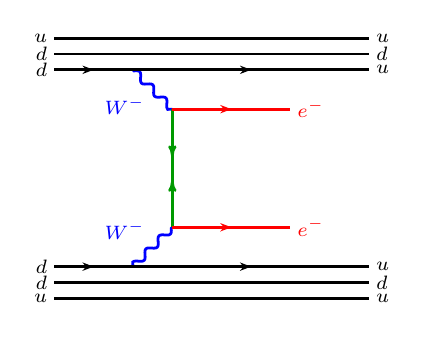
\begin{tikzpicture}\scriptsize
		\newcommand\dy{0.2cm}
		\newcommand\ldx{3cm}
		\newcommand\lsx{1cm}
		\newcommand\hei{0.5cm}
		\newcommand\ange{0.1cm}
		\newcommand\lene{1.5cm}
		\tikzfeynmanset{
		every diagram = small,
		every edge/.style = {line width = 1pt},
		myfermion/.style={
			/tikz/postaction={
				/tikz/decoration={
					markings,
					mark=at position 0.5 with {
						\arrow{Stealth[length=4pt, width=3pt]};
					},
				},
			/tikz/decorate=true,
			},
		},
		mymajorana/.style={
			/tikz/postaction={
				/tikz/decoration={
					markings,
					mark=at position 0.4 with {
						\arrow{>[length=4pt, width=3pt]};
					},
					mark=at position 0.7 with {
						\arrow{<[length=4pt, width=3pt]};
					},
				},
			/tikz/decorate=true,
			},
		},
	}
	\begin{feynman}
		\vertex (b);
		\vertex [below=\hei+1cm of b] (c);
		\vertex [below left=\hei and \hei of c] (d);
		\vertex [above left=\hei and \hei of b] (a);
		% spectator quarks vertices
		\vertex [above=\dy of a] (e);
		\vertex [above=\dy of e] (f);
		\vertex [below=\dy of d] (g);
		\vertex [below=\dy of g] (h);
		% external legs
		\vertex [left=\lsx of a] (i1) {$d$};
		\vertex [left=\lsx of d] (i2) {$d$};
		\vertex [right=\ldx of a] (f1) {$u$};
		\vertex [right=\lene of b] (f2) {\color{red}$e^-$};
		%\vertex [below right=\ange and \lene of b] (f13) {$\bar{\nu}_e$};
		\vertex [right=\lene of c] (f3) {\color{red}$e^-$};
		%\vertex [above right=\ange and \lene of c] (f14) {$\bar{\nu}_e$};
		\vertex [right=\ldx of d] (f4) {$u$};
		% spactator quarks
		\vertex [right=\ldx of e] (f5) {$d$};
		\vertex [left=\lsx of e] (f6) {$d$};
		\vertex [right=\ldx of f] (f7) {$u$};
		\vertex [left=\lsx of f] (f8) {$u$};
		\vertex [right=\ldx of g] (f9) {$d$};
		\vertex [left=\lsx of g] (f10) {$d$};
		\vertex [right=\ldx of h] (f11) {$u$};
		\vertex [left=\lsx of h] (f12) {$u$};

		\diagram* {
			(a) -- [boson, blue, edge label'=$W^-$] (b),
			(c) -- [boson, blue, edge label'=$W^-$] (d),
			(b) -- [mymajorana, green!60!black] (c),
			%(f13) -- [myfermion, green!60!black] (b),
			%(f14) -- [myfermion, green!60!black] (c),
			(i1) -- [myfermion] (a),
			(i2) -- [myfermion] (d),
			(a) -- [myfermion,] (f1),
			(b) -- [myfermion, red] (f2),
			(c) -- [myfermion, red] (f3),
			(d) -- [myfermion] (f4),
			% spectator quarks
			(f6)  -- (e),
			(e)   -- (f5),
			(f8)  -- (f),
			(f)   -- (f7),
			(f10) -- (g),
			(g)   -- (f9),
			(f12) -- (h),
			(h)   -- (f11),

		};
		\end{feynman}
	\end{tikzpicture}
	\column{0.65\textwidth}
%	\begin{exampleblock}{I neutrini oltre il Modello Standard}
%		Il neutrino è una particella di \alert{Majorana} o di \alert{Dirac}?
%	\end{exampleblock}
	\begin{itemize}
		\item {\gerda}: ricerca decadimento doppio-beta senza neutrini (\alert{$0\nbb$}) dell'isotopo \alert{\ce{^76Ge}}
		\item Array di rivelatori arricchiti al \ce{^76Ge} \\ $\longmapsto$ \alert{rivelatore = sorgente}
		\item \alert{Fase II}
			\begin{itemize}
				\item aumento della quantità di \ce{^76Ge}
				\item aggiornamento della strumentazione
			\end{itemize}
			$\longmapsto$ migliore discriminazione del fondo.
	\end{itemize}
	\end{columns}
\end{frame}
\begin{frame}[plain, label=2]{The \alert{GER}manium \alert{D}etector \alert{A}rray}
	\begin{tikzpicture}[fill=white]
	\node at (0,0) {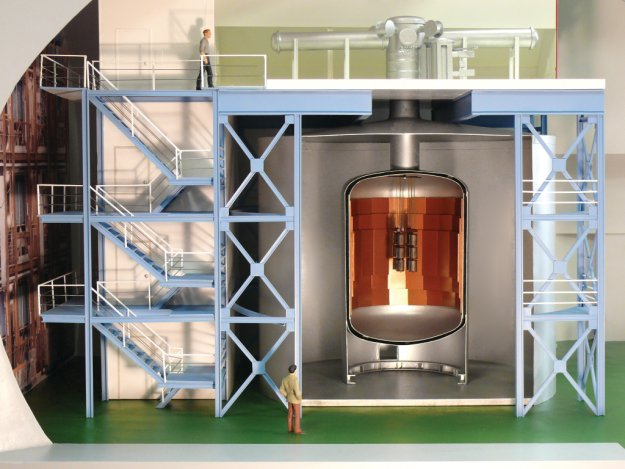
\includegraphics[width=\columnwidth]{../img/GERDAmodel.jpg}}; % CHE IMMAGINE DI MERDA
	\node(e) at (4,3.5) [rectangle,draw,fill] {\textsc{scintillatori}};
	\draw[thick,red,->] (e.south) .. controls +(0,-1) and +(0,1) .. (3,2.6);
	\node(a) at (1.6,-1.2) [rectangle,draw,fill] {LAr};
	\node(b) at (4,1.6) [rectangle,draw,fill] {\textsc{rivelatori} \ce{^76Ge}};
	\draw[thick,red,->] (b.south) .. controls +(0,0) and +(1,0) .. (1.9,-0.4);
	\node(c) at (-1.5,1.6) [rectangle,draw,fill] {\ce{H2O}};
	\draw[thick,red,->] (c.south) .. controls +(0,0) and +(-1,0) .. (0,-1);
	\node(d) at (0,3) [rectangle,draw,fill] {\textsc{schermatura} Cu};
	\draw[thick,red,->] (d.south) .. controls +(0,0) and +(-1,0) .. (1,0);
	%\node at (-3.4,-3.25) {\includegraphics[scale=0.1]{img/logoLNGS.jpg}};
	\node at (-1.65,-3.73) [rectangle,draw=mLightBrown, fill=white] {@ Laboratori Nazionali del Gran Sasso [LNGS]};
	\end{tikzpicture}
\end{frame}
\begin{frame}[label=4]{Oltre il Modello Standard}
	\metroset{block=fill}
	\begin{itemize}
		\item Molte teorie candidate a descrivere la Gravità Quantistica prevedono la rottura spontanea (alla scala di Planck) della simmetria di Lorentz $\longmapsto$ \alert{Standard Model Extension (SME)}.
		\item La scala di energia di Planck è attualmente non accessibile per via sperimentale $\longmapsto$ ricerca a energie minori di \alert{segnali soppressi}.
		\item Questo tipo di rottura spontanea può essere studiata nel settore dei neutrini.
	\end{itemize}
	\begin{alertblock}{Proposta}
		È possibile ricercare effetti di violazione della simmetria di Lorentz nei dati di \alert{$2\nbb$} (\textbf{non} $0\nbb$!) raccolti da {\gerda}
	\end{alertblock}
\end{frame}
\begin{frame}[label=5]{\textit{Lorentz-violating} \texorpdfstring{2$\nbb$}{2nbb} per l'isotopo \ce{^76Ge}}
	\begin{columns}
		\column{0.5\textwidth}
	\begin{center}(\textit{Standard Model} $2\nbb$)\end{center}
		\[\ce{^76Ge}\longmapsto\ce{^76Se}+2e^-+2\bar{\nu}_e\]
	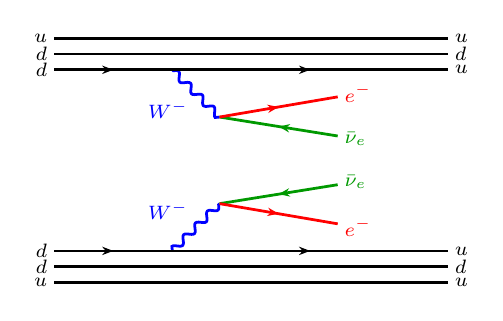
\begin{tikzpicture}
	\scriptsize
	\newcommand\dy{0.2cm}
	\newcommand\ldx{3.5cm}
	\newcommand\lsx{1.5cm}
	\newcommand\hei{0.6cm}
	\newcommand\ange{0.1cm}
	\newcommand\lene{1.5cm}
	\tikzfeynmanset{
		every diagram = small,
		every edge/.style = {line width = 1pt},
		myfermion/.style={
			/tikz/postaction={
				/tikz/decoration={
					markings,
					mark=at position 0.5 with {
						\arrow{Stealth[length=4pt, width=3pt]};
					},
				},
			/tikz/decorate=true,
			},
		},
	}
		\begin{feynman}
			\vertex (b);
			\vertex [below=\hei+0.5cm of b] (c);
			\vertex [below left=\hei and \hei of c] (d);
			\vertex [above left=\hei and \hei of b] (a);
			% spectator quarks vertices
			\vertex [above=\dy of a] (e);
			\vertex [above=\dy of e] (f);
			\vertex [below=\dy of d] (g);
			\vertex [below=\dy of g] (h);
			% external legs
			\vertex [left=\lsx of a] (i1) {$d$};
			\vertex [left=\lsx of d] (i2) {$d$};
			\vertex [right=\ldx of a] (f1) {$u$};
			\vertex [above right=\ange and \lene of b] (f2) {\color{red}$e^-$};
			\vertex [below right=\ange and \lene of b] (f13) {\color{green!60!black}$\bar{\nu}_e$};
			\vertex [below right=\ange and \lene of c] (f3) {\color{red}$e^-$};
			\vertex [above right=\ange and \lene of c] (f14) {\color{green!60!black}$\bar{\nu}_e$};
			\vertex [right=\ldx of d] (f4) {$u$};
			% spactator quarks
			\vertex [right=\ldx of e] (f5) {$d$};
			\vertex [left=\lsx of e] (f6) {$d$};
			\vertex [right=\ldx of f] (f7) {$u$};
			\vertex [left=\lsx of f] (f8) {$u$};
			\vertex [right=\ldx of g] (f9) {$d$};
			\vertex [left=\lsx of g] (f10) {$d$};
			\vertex [right=\ldx of h] (f11) {$u$};
			\vertex [left=\lsx of h] (f12) {$u$};

			\diagram* {
				(a) -- [boson, blue, edge label'=$W^-$] (b),
				(c) -- [boson, blue, edge label'=$W^-$] (d),
				(f13) -- [myfermion, green!60!black] (b),
				(f14) -- [myfermion, green!60!black] (c),
				(i1) -- [myfermion] (a),
				(i2) -- [myfermion] (d),
				(a) -- [myfermion,] (f1),
				(b) -- [myfermion, red] (f2),
				(c) -- [myfermion, red] (f3),
				(d) -- [myfermion] (f4),
				% spectator quarks
				(f6)  -- (e),
				(e)   -- (f5),
				(f8)  -- (f),
				(f)   -- (f7),
				(f10) -- (g),
				(g)   -- (f9),
				(f12) -- (h),
				(h)   -- (f11),
		};
		\end{feynman}
	\end{tikzpicture}
		\column{0.5\textwidth}
	\begin{simpleblock}\alert{\textit{Lorentz-violating} $2\nbb$}\end{simpleblock}
		Distorsione dello spettro in energia ($K=K_1+K_2$) dei due elettroni in uscita.
		\vspace{0.2cm}
	\begin{center}\alert{Distorsione regolata dal coefficiente $\aof$}\end{center}
		\alert{\[\frac{\text{d}\Gamma_{TOT}}{\text{d}K}=\frac{\text{d}\Gamma}{\text{d}K}+\frac{\text{d}\delta\Gamma}{\text{d}K}\]}
	\end{columns}
\end{frame}
\begin{frame}[label=6]{Lo spettro in energia del \texorpdfstring{2$\nbb$}{2nbb}}
	\begin{columns}
		\column{0.5\textwidth}
			\metroset{block=fill}
			\begin{exampleblock}{\textit{Standard-Model} $2\nbb$}
			\[\begin{split}
					\frac{\text{d}\Gamma}{\text{d}K} &=C(K^5+10K^4+40K^3+ \\
						&+60K^2+30){\color{blue}(Q_{\beta\beta}-K)^5}
			\end{split}\]
			\end{exampleblock}
			\uncover<2->{%
				\begin{exampleblock}{\textit{Lorentz-violating} $2\nbb$}
					\[\begin{split}
						\frac{\text{d}\delta\Gamma}{\text{d}K} &=C(K^5+10K^4+40K^3+ \\
							&+60K^2+30){\color{red}10\aof(Q_{\beta\beta}-K)^4}
					\end{split}\]
				\end{exampleblock}
			}
		\column{0.5\textwidth}
			\vspace{1cm}
			\begin{center}
				\begin{adjustbox}{scale=1.2}
				\begin{tikzpicture}
					\begin{axis}[
								mlineplot,
								width=\textwidth, height=6cm,
								xmin=0, xmax=4.5,
								ymin=0, ymax=0.6,
								samples=200,
								xlabel=Energy/$m_e$,
								yticklabels={,,}
								ylabel=a.u.
								]
						\only<1>{
							\addplot [mark=none, color=red, opacity=.1, line width=1pt, domain=0:4] 
								{x*(4-x)^4*((x)^4+10*(x)^3+40*(x)^2+60*(x)+30)/27814};
						}
						\only<2->{
							\addplot [mark=none, color=red, line width=1pt, domain=0:4] 
								{x*(4-x)^4*((x)^4+10*(x)^3+40*(x)^2+60*(x)+30)/27814};
						}
						\addplot [mark=none, color=blue, line width=1pt, domain=0:4] 
							{x*(4-x)^5*((x)^4+10*(x)^3+40*(x)^2+60*(x)+30)/65749};
						%\node[pin=30:{$2\nu\beta\beta$}] at (axis cs:2,2.3) {};
						%\addplot [mark=none, color=blue, line width=1pt, domain=4:5] {0};
						%\node[pin=90:{$0\nu\beta\beta$}] at (axis cs:4,0.8) {};
					\end{axis}
				\end{tikzpicture}
				\end{adjustbox}
			\end{center}
	\end{columns}
\end{frame}
\begin{frame}[label=7]
	\metroset{block=fill}
	\begin{alertblock}{Obiettivo}
		Estrarre una stima di $\aof$ dai dati di {\gerda} -- Fase II tramite un'analisi statistica Bayesiana
	\end{alertblock}
	Preparazione all'analisi statistica:
	\begin{itemize}
		\item Applicazione dei \alert{tagli di qualità} sui dati.
		\item Costruzione del \alert{modello di fondo}: produzione delle simulazioni Monte Carlo.
		\item Costruzione del \alert{modello statistico} utilizzato per interpolare i dati con le simulazioni.
	\end{itemize}
\end{frame}
\begin{frame}[label=8]{Tagli di qualità}
	È possibile attuare i seguenti tagli di qualità sui dati: eventi corrispondenti a
	\begin{itemize}
		\item \alert{errori di acquisizione o di ricostruzione} delle quantità fisiche associate a una forma d'onda
		\item rilascio di energia nell'acqua o negli scintillatori posti sopra l'apparato (\alert{muon veto})
		\item rilascio di energia in più rivelatori (\alert{coincidenze}) $\longmapsto$ evento di fondo
	\end{itemize}
	sono \textbf{esclusi} dall'analisi.
\end{frame}
\begin{frame}[plain, c, label=9]
	\vspace{0.5cm}
\centerline{%
	\begin{tikzpicture}\scriptsize
	\begin{groupplot}[	group style = { group size = 1 by 2,
										xlabels at = edge bottom,
										xticklabels at = edge bottom,
										ylabels at = edge left,
										vertical sep = 0pt
										},
						width = 12cm,
						height = 5cm,
						xlabel = energy {[keV]},
						%xlabel style = {at={(axis description cs:0.5,0.07)}},
						%ylabel style = {at={(axis description cs:0.02,0.5)}},
						ylabel = counts,
						xmin = 0, xmax = 6000,
						ymin = 0, ymax = 4.7,
						ytick = {0.301,1.301,2.301,3.301,4.301},
						yticklabels = {$10^0$,$10^1$,$10^2$,$10^3$,$10^4$},
						grid = major,
						/pgf/number format/1000 sep={},
						]
		\nextgroupplot
			\addplot[const plot, draw = red] file {../data/BEGe.dat};
			\node at (axis cs:380,3.8) {\ce{^{39}Ar}};
			\node at (axis cs:1400,3.5) {\ce{^{40}K}};
			\node at (axis cs:1500,4) {\ce{^{42}K}};
			\node at (axis cs:2550,2) {\ce{^{208}Tl}};
			\node at (axis cs:2300,1.5) {\ce{^{214}Bi}};
			\node at (axis cs:1700,2) {\ce{^{214}Bi}};
			\node at (axis cs:560,3.1) {\ce{^{214}Bi}};
			\node at (axis cs:850,3.3) {\ce{^{228}Ac}};
			\draw (axis cs:911,3.0) -- (axis cs:911,2.75);
			% alpha
			\node at (axis cs:4700,1.6) {\ce{^{226}Ra}};
			\node at (axis cs:5100,1.9) {\ce{^{210}Po}};
			\node[rectangle,draw,fill=bg] at (axis cs:3500,3.8) {BEGe --- 19.74 kg$\cdot$yr};
			\fill[green, opacity=0.5] (axis cs:2014,0) rectangle (axis cs:2064,4.7);
			\node at (axis cs:5450,3.5) {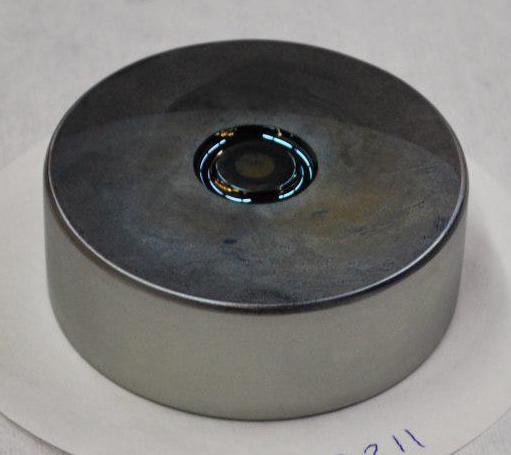
\includegraphics[width=1.5cm]{img/bege_pic.jpg}};
		\nextgroupplot
			\addplot[const plot, draw = blue] file {../data/EnrCoax.dat};
			\node at (axis cs:380,3.8) {\ce{^{39}Ar}};
			\node at (axis cs:1400,3.5) {\ce{^{40}K}};
			\node at (axis cs:1500,4) {\ce{^{42}K}};
			\node at (axis cs:2550,2) {\ce{^{208}Tl}};
			\node at (axis cs:2300,1.3) {\ce{^{214}Bi}};
			\node at (axis cs:560,3) {\ce{^{214}Bi}};
			\node at (axis cs:1700,2) {\ce{^{214}Bi}};
			% alpha
			\node at (axis cs:4700,1.8) {\ce{^{226}Ra}};
			\node at (axis cs:5100,2.1) {\ce{^{210}Po}};
			\node at (axis cs:5400,0.7) {\ce{^{222}Rn}};
			\node at (axis cs:5800,0.7) {\ce{^{218}Po}};
			\node[rectangle,draw,fill=bg] at (axis cs:3500,3.8) {\textsc{enr coax} --- 16.22 kg$\cdot$yr};
			\fill[green, opacity=0.5] (axis cs:2014,0) rectangle (axis cs:2064,4.7);
			\node at (axis cs:5500,3.4) {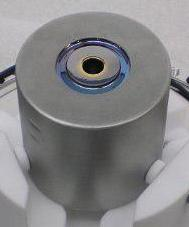
\includegraphics[width=1.3cm]{img/coax_pic.jpg}};
	\end{groupplot}
\end{tikzpicture}%
}
\end{frame}
\begin{frame}[label=10]{Modello di fondo --- simulazioni Monte Carlo}
	La costruzione di un \alert{modello di fondo} è fondamentale per estrarre gli eventi $2\nbb$ dai dati e studiarne lo spettro in energia.

	I cambiamenti apportati in {\gerda} --- Fase II richiedono un modello di fondo aggiornato rispetto ai modelli preesistenti.
	\uncover<2->{
	\begin{itemize}
		\item il \alert{$2\nbb$}, \textit{Standard-Model} e \textit{Lorentz-violating}, simulato nei rivelatori al Germanio
		\item {\color{mLightGreen}misure di screening dei materiali} $\longmapsto$ gli \alert{isotopi}
			\[\ce{^212Bi}, \ce{^214Bi}, \ce{^208Tl}, \ce{^214Pb}, \ce{^40K}, \ce{^42K}, \ce{^60Co}, \ce{^228Ac}, \ce{^234Pa}, \ce{^207Bi},\]
			sono stati simulati all'interno delle varie componenti di {\gerda}
		\item Le sorgenti di particelle $\alpha$ simulate sulla superficie dei rivelatori $\longmapsto$ \alert{\textit{$\alpha$-model}}
	\end{itemize}
}
\end{frame}
\begin{frame}[label=12]{Modello statistico}
	La presenza delle varie componenti simulate è stata indagata con un'\alert{analisi statistica di tipo Bayesiano} (librerie software \texttt{BAT}\footnote{basate su metodi MCMC. \texttt{https://wwwold.mppmu.mpg.de/bat/}}).
	\begin{itemize}
		\item Intervallo di Fit: [570, 5300] keV
		\item gli spettri in energia sommati sui due tipi di rivelatori (\textbf{BEGe e EnrCoax}) mantenuti \textbf{separati} nell'analisi ($\mathcal{L}=\mathcal{L}_1\cdot\mathcal{L}_2$)
		\item \textbf{\textit{binning} variabile} in larghezza studiato per ovviare alle incertezze sulla calibrazione in energia attorno alle linee $\gamma$ più evidenti
		\item \textbf{\textit{prior distributions}} per le attività di alcune sorgenti
		\item \textbf{p-value} per stimare il grado di \textit{goodness-of-fit}
	\end{itemize}
\end{frame}
\begin{frame}[label=16]{Analisi}
	\begin{enumerate}
		\item Modello con il solo $2\nbb$ del Modello Standard
		\begin{enumerate}
			\item Modello massimale con tutte le sorgenti di fondo in tutte le posizioni possibili
			\item Modello minimale con sorgenti ad attività non nulla
			\item Modello minimale con l'aggiunta delle \textit{prior distributions}
		\end{enumerate}
		\item[$\longmapsto$] \alert{Stima della vita media $\Tnu$ dello \textit{Standard-Model} $2\nbb$}
		\item<2-> Modello di cui al punto (1.3) con l'aggiunta del canale \textit{Lorentz-violating} del $2\nbb$
		\item[$\longmapsto$]<2-> \alert{Stima del parametero $\aof$ del \textit{Lorentz-violating} $2\nbb$}
	\end{enumerate}
\end{frame}
\tikzexternaldisable
\section{Risultati}
\tikzexternalenable
\begin{frame}[plain,c,label=20]{Risultati --- modello di fondo}
	\vspace{0.5cm}
	\centerline{\begin{tikzpicture}\scriptsize
	\pgfplotsset{every axis legend/.append style={at={(1.02,1)}, anchor=north west}}
	\begin{groupplot}[group style = { group size = 1 by 2 ,
										xlabels at = edge bottom,
										xticklabels at = edge bottom,
										ylabels at = edge left,
										vertical sep = 0pt
										},
					xmin = 570, xmax = 1800,
					/pgf/number format/1000 sep={},
					ylabel=cts/bin,
					xlabel=energy {[keV]},
					%xlabel style = {at={(axis description cs:0.5,0.07)}},
					%ylabel style = {at={(axis description cs:0.02,0.5)}},
					legend style={fill=bg}
					]
		\nextgroupplot[ytick = {-5,0,5}, yticklabels = {$10^{-5}$,$10^0$,$10^5$},
						width = 10.5cm, height = 7cm,
						ymin = -5,
						%grid = major
						]
			\node[rectangle, draw] at (axis cs:1700,4) {\normalsize BEGe};
			\addplot[const plot, blue] table[x=energy, y=2nbb] {../data/resBEGe.dat};
			\addplot[const plot, black!40!green] table[x=energy, y=K42homLAr] {../data/resBEGe.dat};
			% K40
			\addplot[const plot, orange] table[x=energy, y=K40fibers] {../data/resBEGe.dat};
			\addplot[const plot, violet] table[x=energy, y=K40holder] {../data/resBEGe.dat};
			\addplot[const plot, ] table[x=energy, y=K40cables] {../data/resBEGe.dat};
			%alpha
			\addplot[const plot, red, densely dashdotted] table[x=energy, y=alpha] {../data/resBEGe.dat};
			\addplot[only marks, mark size = 0.5pt] table[x=midenergy, y=data] {../data/resBEGe.dat};
			\addplot[const plot, red, thick] table[x=energy, y=sum] {../data/resBEGe.dat};
			% legend
				\addlegendentry{$2\nu\beta\beta$}
				\addlegendentry{\ce{^{42}K} \textsc{[homLAr]}};
				\addlegendentry{\ce{^{40}K} \textsc{[f]}}
				\addlegendentry{\ce{^{40}K} \textsc{[h]}}
				\addlegendentry{\ce{^{40}K} \textsc{[c]}}
				\addlegendentry{$\alpha$-model}
				\addlegendentry{Data}
				\addlegendentry{Total}
		\nextgroupplot[width = 10.5cm, height = 3cm, enlargelimits=false]
			\addplot[const plot, orange!70, draw=none, name path = A] table[x=energy, y=3sig] {../data/residualsBEGe.dat};
			\addplot[const plot, orange!70, draw=none, name path = B] table[x=energy, y=-3sig] {../data/residualsBEGe.dat};
			\addplot[orange!70] fill between[of=A and B];
			\addplot[const plot, yellow!70, draw=none, name path = C] table[x=energy, y=2sig] {../data/residualsBEGe.dat};
			\addplot[const plot, yellow!70, draw=none, name path = D] table[x=energy, y=-2sig] {../data/residualsBEGe.dat};
			\addplot[yellow!70] fill between[of=C and D];
			\addplot[const plot, green!70, draw=none, name path = E] table[x=energy, y=1sig] {../data/residualsBEGe.dat};
			\addplot[const plot, green!70, draw=none, name path = F] table[x=energy, y=-1sig] {../data/residualsBEGe.dat};
			\addplot[green!70] fill between[of=E and F];
			\addplot[only marks, mark size=0.5pt] table[x=midenergy, y=res] {../data/residualsBEGe.dat};
	\end{groupplot}
\end{tikzpicture}}
\end{frame}
\begin{frame}[plain,c,label=21]{Risultati --- modello di fondo}
	\vspace{0.5cm}
	\centerline{\begin{tikzpicture}\scriptsize
\pgfplotsset{every axis legend/.append style={at={(1.02,1)}, anchor=north west}}
	\begin{groupplot}[group style = { group size = 1 by 2 ,
										xlabels at = edge bottom,
										xticklabels at = edge bottom,
										ylabels at = edge left,
										vertical sep = 0pt
										},
					xmin = 570, xmax = 1800,
					/pgf/number format/1000 sep={},
					ylabel=cts/bin,
					xlabel=energy {[keV]},
					%xlabel style = {at={(axis description cs:0.5,0.07)}},
					%ylabel style = {at={(axis description cs:0.02,0.5)}},
					legend style={fill=bg}
					]
		\nextgroupplot[ytick = {-5,0,5}, yticklabels = {$10^{-5}$,$10^0$,$10^5$},
						width = 10cm, height = 7cm,
						ymin = -9,
						%grid = major
						]
			\node[rectangle, draw] at (axis cs:1700,4) {\normalsize BEGe};
			\addplot[const plot, blue] table[x=energy, y=2nbb] {../data/resBEGe.dat};
			% Bi212Tl208
			\addplot[const plot, green!50!black] table[x=energy, y=Bi212Tl208fibers] {../data/resBEGe.dat};
			\addplot[const plot, orange] table[x=energy, y=Bi212Tl208cables] {../data/resBEGe.dat};
			% Pb214Bi214
			\addplot[const plot, violet] table[x=energy, y=Pb214Bi214fibers] {../data/resBEGe.dat};
			\addplot[const plot, ] table[x=energy, y=Pb214Bi214holder] {../data/resBEGe.dat};
			%alpha
			\addplot[only marks, mark size = 0.5pt] table[x=midenergy, y=data] {../data/resBEGe.dat};
			\addplot[const plot, red, thick] table[x=energy, y=sum] {../data/resBEGe.dat};
			% legend
				\addlegendentry{$2\nu\beta\beta$}
				\addlegendentry{\ce{^{214}Bi} + \ce{^{214}Pb} \textsc{[f]}}
				\addlegendentry{\ce{^{214}Bi} + \ce{^{214}Pb} \textsc{[c]}}
				\addlegendentry{\ce{^{212}Bi} + \ce{^{208}Tl} \textsc{[f]}}
				\addlegendentry{\ce{^{212}Bi} + \ce{^{208}Tl} \textsc{[h]}}
				\addlegendentry{Data}
				\addlegendentry{Total}
		\nextgroupplot[width = 10cm, height = 3cm, enlargelimits=false]
			\addplot[const plot, orange!70, draw=none, name path = A] table[x=energy, y=3sig] {../data/residualsBEGe.dat};
			\addplot[const plot, orange!70, draw=none, name path = B] table[x=energy, y=-3sig] {../data/residualsBEGe.dat};
			\addplot[orange!70] fill between[of=A and B];
			\addplot[const plot, yellow!70, draw=none, name path = C] table[x=energy, y=2sig] {../data/residualsBEGe.dat};
			\addplot[const plot, yellow!70, draw=none, name path = D] table[x=energy, y=-2sig] {../data/residualsBEGe.dat};
			\addplot[yellow!70] fill between[of=C and D];
			\addplot[const plot, green!70, draw=none, name path = E] table[x=energy, y=1sig] {../data/residualsBEGe.dat};
			\addplot[const plot, green!70, draw=none, name path = F] table[x=energy, y=-1sig] {../data/residualsBEGe.dat};
			\addplot[green!70] fill between[of=E and F];
			\addplot[only marks, mark size=0.5pt] table[x=midenergy, y=res] {../data/residualsBEGe.dat};
	\end{groupplot}
\end{tikzpicture}}
\end{frame}
\begin{frame}[plain,c,label=22]{Risultati --- modello di fondo}
	\vspace{0.5cm}
	\centerline{\begin{tikzpicture}\scriptsize
	\pgfplotsset{every axis legend/.append style={at={(1.02,1)}, anchor=north west}}
	\begin{groupplot}[group style = { group size = 1 by 2 ,
										xlabels at = edge bottom,
										xticklabels at = edge bottom,
										ylabels at = edge left,
										vertical sep = 0pt
										},
					xmin = 570, xmax = 1800,
					/pgf/number format/1000 sep={},
					ylabel=cts/bin,
					xlabel=energy {[keV]},
					%xlabel style = {at={(axis description cs:0.5,0.07)}},
					%ylabel style = {at={(axis description cs:0.02,0.5)}},
					legend style={fill=bg}
					]
		\nextgroupplot[ytick = {-5,0,5}, yticklabels = {$10^{-5}$,$10^0$,$10^5$},
						width = 10.5cm, height = 7cm,
						ymin = -9,
						%grid = major
						]
			\node[rectangle, draw] at (axis cs:1700,4) {\normalsize BEGe};
			\addplot[const plot, blue] table[x=energy, y=2nbb] {../data/resBEGe.dat};
			% other
			\addplot[const plot, orange] table[x=energy, y=Ac228holder] {../data/resBEGe.dat};
			\addplot[const plot, green!50!black] table[x=energy, y=Co60holder] {../data/resBEGe.dat};
			\addplot[const plot, violet] table[x=energy, y=Pa234cables] {../data/resBEGe.dat};
			\addplot[const plot, ] table[x=energy, y=Bi207minishroud] {../data/resBEGe.dat};
			%alpha
			\addplot[only marks, mark size = 0.5pt] table[x=midenergy, y=data] {../data/resBEGe.dat};
			\addplot[const plot, red, thick] table[x=energy, y=sum] {../data/resBEGe.dat};
			% legend
				\addlegendentry{$2\nu\beta\beta$}
				\addlegendentry{\ce{^{228}Ac} \textsc{[h]}}
				\addlegendentry{\ce{^{60}Co} \textsc{[h]}}
				\addlegendentry{\ce{^{234\text{m}}Pa} \textsc{[c]}}
				\addlegendentry{\ce{^{207}Bi} \textsc{[ms]}}
				%\addlegendentry{$\alpha$-model}
				\addlegendentry{Data}
				\addlegendentry{Total}
		\nextgroupplot[width = 10.5cm, height = 3cm, enlargelimits=false]
			\addplot[const plot, orange!70, draw=none, name path = A] table[x=energy, y=3sig] {../data/residualsBEGe.dat};
			\addplot[const plot, orange!70, draw=none, name path = B] table[x=energy, y=-3sig] {../data/residualsBEGe.dat};
			\addplot[orange!70] fill between[of=A and B];
			\addplot[const plot, yellow!70, draw=none, name path = C] table[x=energy, y=2sig] {../data/residualsBEGe.dat};
			\addplot[const plot, yellow!70, draw=none, name path = D] table[x=energy, y=-2sig] {../data/residualsBEGe.dat};
			\addplot[yellow!70] fill between[of=C and D];
			\addplot[const plot, green!70, draw=none, name path = E] table[x=energy, y=1sig] {../data/residualsBEGe.dat};
			\addplot[const plot, green!70, draw=none, name path = F] table[x=energy, y=-1sig] {../data/residualsBEGe.dat};
			\addplot[green!70] fill between[of=E and F];
			\addplot[only marks, mark size=0.5pt] table[x=midenergy, y=res] {../data/residualsBEGe.dat};
	\end{groupplot}
\end{tikzpicture}}
\end{frame}
\begin{frame}[label=13]{Risultati --- \texorpdfstring{$\Tnu$}{Tnu}}
		\begin{center}
		\begin{tikzpicture}\small
			\begin{axis}[grid = major,
				/pgf/number format/1000 sep={},
				xmin = 0.49, xmax = 0.53,
				ymin = 0,% ymax = 1.0E04,
				%xlabel style = {at={(axis description cs:0.5,0.02)}},
				%ylabel style = {at={(axis description cs:0.15,0.5)}},
				height = 5cm,
				xlabel = {$1/T_{1/2}^{2\nu}$ $[10^{-21}\;\text{yr}^{-1}]$},
				width = 8cm,
				ylabel = counts,
				legend entries = {\textit{prior}, \textit{posterior}},
				legend style={fill=bg}
				]
				\addplot[const plot, draw = blue] table[x=point, y=prior] {../data/2nbb_post.dat};
				\addplot[const plot, draw = red] table[x=point, y=post] {../data/2nbb_post.dat};
			\end{axis}
		\end{tikzpicture}
		\end{center}
		\begin{tcolorbox}[ams align*,
							boxsep=0.25ex,
							arc=0ex,
							opacityframe=.6,
							opacityback=.6,
							colback=bg!80!fg,
							colframe=white,
							boxrule=0pt,
							]
					\Tnu &=({1.984\;\;^{+0.020}_{-0.020\:\text{stat}}}\;\;{^{+0.098}_{-0.075\:\text{sys}}})\cdot10^{21}\;\text{yr}\\%
						 &=(1.98\;\;^{+0.10}_{-0.08})\cdot10^{21}\;\text{yr}
		\end{tcolorbox}
\end{frame}
\begin{frame}[label=17]{Risultati --- \texorpdfstring{$\aof$}{aof}}
	\metroset{block=fill}
	\begin{columns}
		\column{0.5\textwidth}
		\begin{itemize}
			\item La moda è compatibile con zero al 90\% C.I.
			\item Convoluzione con la distribuzione delle {\color{mLightGreen}incertezze sistematiche}.
		\end{itemize}
		\vspace{0.6cm}
		\begin{simpleblock}
			\alert{$\aof<7.5\cdot10^{-8}\ \text{GeV}\ (\text{90\% C.I.})$}
		\end{simpleblock}
		\column{0.5\textwidth}
		\vspace{1cm}
		\begin{tikzpicture}\scriptsize
			\begin{axis}[
				width = 6cm,
				height = 7cm,
				xlabel = {$\mathring{a}_\text{of}^{(3)}/m_e$},
				%xlabel style = {at={(axis description cs:0.5,0.05)}},
				%ylabel style = {at={(axis description cs:0.03,0.5)}},
				ylabel = counts,
				xmin = 0, xmax = 3E-04,
				%domain=0:0.0004, restrict y to domain=0:12000,
				ymin = 0,% ymax = 1.0E04,
				xtick = {0,0.0001,0.0002,0.0003,0.0004},
				grid = major,
				/pgf/number format/1000 sep={},
				legend entries = {original, folded},
				legend style={fill=bg}
				]
				\addplot[const plot, draw = black, densely dashdotted] table[x=aof, y=counts] {../data/aof.dat};
				\addplot[const plot, draw = red] table[x=aof, y=countsmear] {../data/aof.dat};
				\draw[red] (axis cs:1.46e-04,0) -- (axis cs:1.46E-04,2.7E03);
				\draw[densely dashdotted] (axis cs:1.44e-04,0) -- (axis cs:1.44E-04,2.8E03);
			\end{axis}
		\end{tikzpicture}
	\end{columns}
\end{frame}
\begin{frame}[plain,c,label=18]{Risultati --- \texorpdfstring{$2\nbb$}{2nbb}}
	\only<1-2>{
	\centerline{\begin{tikzpicture}\small%
		\begin{axis}[xmin = 570, xmax = 2000,
				ymin = -1,
				width = 12cm, height = 7cm,
				/pgf/number format/1000 sep={},
				ylabel=counts/bin,
				xlabel=energy {[keV]},
				%xlabel style = {at={(axis description cs:0.5,0.03)}},
				ylabel style = {at={(axis description cs:-0.05,0.5)}},
				ytick = {-1,0,1,2},
				yticklabels = {0,1,10,100},
				legend style={fill=bg}
				]
			\addplot[const plot] table[x=low, y=data] {../data/double_beta.dat};
			\addplot[const plot, black!50!green] table[x=low, y=2nbbLV] {../data/double_beta.dat};
			\addplot[const plot, blue] table[x=low, y=2nbb] {../data/double_beta.dat};
			\only<2->{\addplot[const plot, red] table[x=low, y=2nbb+] {../data/double_beta.dat};}
			% legend
				\addlegendentry{BEGe data};
				\addlegendentry{$2\nu\beta\beta$LV};
				\addlegendentry{$2\nu\beta\beta$};
				\only<2->{\addlegendentry{$2\nu\beta\beta$+$2\nu\beta\beta$LV};}
		\end{axis}%
	\end{tikzpicture}}
	}
\end{frame}
\begin{frame}[label=19]{Precedenti stime}
	\metroset{block=fill}
	\begin{exampleblock}{$\Tnu=(1.98\;\;^{+0.10}_{-0.08})\cdot10^{21}$ yr}
		\begin{itemize}
			\item \textbf{{\gerda} -- Fase I:} $(1.926\pm0.094)\cdot10^{21}$ yr \\ {\footnotesize Agostini M.~et al.~\textit{Eur.~Phys.~J.~C75(9):416}, 2015}
		\end{itemize}
	\end{exampleblock}
	\begin{exampleblock}{$\aof<7.5\cdot10^{-8}$ GeV (90\% C.I.)}
		\begin{itemize}
			\item \textbf{Analisi a posteriori su decadimento-$\beta$:} $\aof\lesssim1\cdot10^{-9}$ GeV \\ {\footnotesize Díaz J.S.~et al.~\textit{Phys.~Rev.~D88(7):071902}, 2013}
			\item \textbf{EXO-200:} $\aof\lesssim7.6\cdot10^{-6}$ GeV \\ {\footnotesize Albert J.B.~et al.~\textit{Phys.~Rev.~D.~93:072001}, 2016}
		\end{itemize}
	\end{exampleblock}
\end{frame}
\begin{frame}[label=26]{Conclusioni}
	\metroset{block=fill}
	\begin{alertblock}{Obiettivo}
		Ricerca di effetti \textit{Lorentz-violating} nei dati $2\nbb$ di {\gerda} \\ $\longmapsto$ valutazione della distorsione dello spettro in energia regolata da $\aof$.
	\end{alertblock}
	Tramite:
	\begin{itemize}
		\item un \alert{modello di fondo aggiornato} alla Fase II di {\gerda};
		\item l'implementazione di un'analisi statistica Bayesiana.
	\end{itemize}
	Risultati (comprensivi delle incertezze sistematiche):
	\[\Tnu=(1.98\;\;^{+0.10}_{-0.08})\cdot10^{21}\ \text{yr ,}\qquad\aof<7.5\cdot10^{-8}\ \text{GeV (90\% C.I.)}\]
	confrontati con precedenti stime presenti in letteratura.
\end{frame}
\appendix
\begin{frame}[standout, label=14]
	Backup
\end{frame}
\begin{frame}[label=30]{\textit{Binning}}
	\begin{table}
	\centering
	\begin{tabular}{lcc}
		\toprule
		Source	&	Line [keV]	&	bin size [keV]	\\
		\midrule
		\ce{^{42}K}	&	1461	&	12	\\
		\ce{^{40}K}	&	1525	&	12	\\
		\ce{^{208}Tl}	&	2614	&	12	\\
		\cmidrule{1-3}
		\multirow{4}{*}{\ce{^{214}Bi}}	&	609		&	12	\\
			&	1764	&	8	\\
			&	2204	&	8	\\
			&	2247	&	12	\\
		\cmidrule{1-3}
		else	&		&	4	\\
		\bottomrule
	\end{tabular}
\end{table}
\end{frame}
\begin{frame}[label=15]{Sistematiche}
	Singoli contributi alle incertezze sistematiche su $\Tnu$ e sul 90° quantile della \textit{posterior distribution} di $\aof$
	\begin{table}
	\centering
	{\renewcommand{\arraystretch}{1.1}
	\begin{tabular}{lcc}
			\toprule
			Contributo					&	$\Tnu$ [\%]			&$\aof$ [\%]			\\
			\midrule
			\textit{Binning}							&	$\pm$1.2		&$\pm$14.3			\\
			MC geometria						&	\multicolumn{2}{c}{$\pm$1.0}				\\
			MC \textsc{Geant4}						&	\multicolumn{2}{c}{$\pm$2.0}				\\
			Frazione di massa attiva 			&	$^{+3.9}_{-2.5}$	&	$^{+3.8}_{-1.7}$	\\
			Frazione di arricchimento				&	$^{+2.0}_{-1.6}$	&	$^{+2.0}_{-1.8}$	\\
			Acquisizione e selezione dati	&	\multicolumn{2}{c}{$\pm0.5$}			\\
			\midrule
			Totale							&	$^{+5.1}_{-3.9}$	&$^{+15.1}_{-14.7}$	\\
			\bottomrule
	\end{tabular}}
\end{table}
\end{frame}
\begin{frame}[plain,c,label=27]{Simulazioni Monte Carlo --- Volumi}
%	\begin{figure}[t]
%	\centering
	\begin{center}
	\resizebox{9cm}{!}{%
		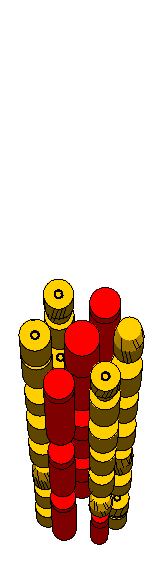
\includegraphics{../img/gedet.pdf}%
		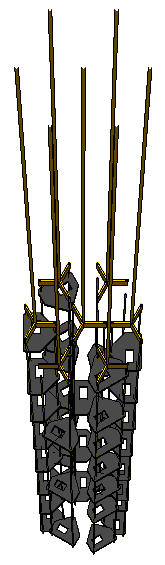
\includegraphics{../img/holders.pdf}%
		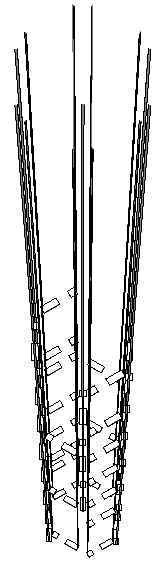
\includegraphics{../img/cables.pdf}%
		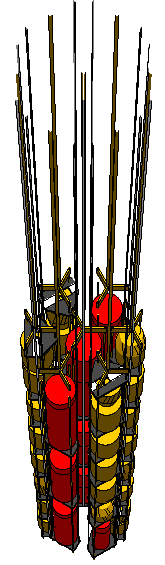
\includegraphics{../img/all.pdf}%
	}%
	\end{center}
%	\caption{Implementation of the simulated volumes in \textsc{MaGe}. From left to right: the germanium detectors, the holder mounting, the cables and the three volumes put together.}\label{fig:volumes}
%\end{figure}
\end{frame}
\begin{frame}[plain, label=11]{Simulazioni Monte Carlo --- Summary}
\begin{table}\small
	\centerline{%
	\begin{tabular}{rccccccc}
		\toprule
						&	Holders	&	Cables	&	Mini-shroud	&	Fibers	&	Contacts	&	LAr	&	Ge\\
		\midrule
		$2\nbb$			&	&	&	&	&	&	&	\checkmark\\
		$2\nbb$LV		&	&	&	&	&	&	&	\checkmark\\
		\ce{^{42}K}		&	&	&	&	&	\checkmark&	\checkmark&	\\
		\ce{^{40}K}		&	&	\checkmark&	\checkmark&	\checkmark&	\checkmark&	&	\\
		\ce{^{214}Bi}	&	\checkmark&	\checkmark&	\checkmark&	\checkmark&	&	&\\
		\ce{^{214}Pb}	&	\checkmark&	\checkmark&	\checkmark&	\checkmark&	&	&\\
		\ce{^{234\text{m}}Pa}	&	\checkmark&	&	\checkmark&	&	\checkmark&	&\\
		\ce{^{212}Bi}	&	\checkmark&	\checkmark&	\checkmark&	\checkmark&	&	&\\
		\ce{^{208}Tl}	&	\checkmark&	\checkmark&	\checkmark&	\checkmark&	&	&\\
		\ce{^{228}Ac}	&	\checkmark&	&	&	&	&	&	\\
		\ce{^{60}Co}	&	\checkmark&	&	&	&	&	&	\\
		\ce{^{207}Bi}	&	\checkmark&	\checkmark&	\checkmark&	&	&	&	\\
		$\alpha$-model	&	&	&	&	&	&	\checkmark&	\\
		\bottomrule
	\end{tabular}%
}%
\end{table}
\end{frame}
\begin{frame}[label=28]{Statistica Bayesiana}
	Learning from experiment:
	\[P_{i+1}(\vec{\lambda},\vec{\nu},M\mid\vec{D})=\frac{f(\vec{x}=\vec{D}\mid\vec{\lambda},\vec{\nu},M)P_i(\vec{\lambda},\vec{\nu},M)}{\sum_M\int f(\vec{x}=\vec{D}\mid\vec{\lambda},\vec{\nu},M)P_i(\vec{\lambda},\vec{\nu},M)}\]
	Parameter estimation:
	\[P(\vec{\lambda},\vec{\nu}\mid\vec{D},M)=\frac{P(\vec{x}=\vec{D}\mid\vec{\lambda},\vec{\nu},M)P_0(\vec{\lambda},\vec{\nu}\mid M)}{\int P(\vec{x}=\vec{D}\mid\vec{\lambda},\vec{\nu},M)P_0(\vec{\lambda},\vec{\nu}\mid M)}\]
	Marginalized posterior:
	\[P(\lambda_i\mid\vec{D},M)=\int P(\vec{\lambda},\vec{\nu}\mid\vec{D},M)\text{d}\vec{\lambda}_{i\neq j}\text{d}\vec{\nu}\]
\end{frame}
\begin{frame}[label=29]{Likelihood}
	\[P(\vec{D}\mid\vec{\lambda})=P_\text{BEGe}(\vec{D}\mid\vec{\lambda})P_\textsc{coax}(\vec{D}\mid\vec{\lambda})=\prod_i^N\left[\frac{e^{-\mu_i}\mu_i^{n_i}}{n_i!}\right]_\text{BEGe}\prod_j^N\left[\frac{e^{-\mu_j}\mu_j^{n_j}}{n_j!}\right]_\textsc{coax}\]
\end{frame}
\begin{frame}[plain,c,label=23]{Risultati --- modello di fondo}
	\vspace{0.5cm}
	\centerline{\begin{tikzpicture}\scriptsize
	\pgfplotsset{every axis legend/.append style={at={(1.02,1)}, anchor=north west}}
	\begin{groupplot}[group style = { group size = 1 by 2 ,
										xlabels at = edge bottom,
										xticklabels at = edge bottom,
										ylabels at = edge left,
										vertical sep = 0pt
										},
					xmin = 1800, xmax = 3500,
					/pgf/number format/1000 sep={},
					ylabel=cts/bin,
					xlabel=energy {[keV]},
					%xlabel style = {at={(axis description cs:0.5,0.07)}},
					%ylabel style = {at={(axis description cs:0.015,0.5)}},
					domain = 570:5300, restrict y to domain = -1000:1000,
					legend style={fill=bg}
					]
					\nextgroupplot[ytick = {-10,-5,0,5}, yticklabels = {$10^{-10}$,$10^{-5}$,$10^0$,$10^5$},
						width = 10.5cm, height = 7cm,
						ymin = -13,
						%grid = major
						]
			\node[rectangle, draw] at (axis cs:3400,-7) {\normalsize BEGe};
			\addplot[const plot, blue] table[x=energy, y=2nbb] {../data/resBEGe.dat};
			\addplot[const plot, black!50!green] table[x=energy, y=K42homLAr] {../data/resBEGe.dat};
			% other
			\addplot[const plot, orange] table[x=energy, y=Ac228holder] {../data/resBEGe.dat};
			\addplot[const plot, violet] table[x=energy, y=Co60holder] {../data/resBEGe.dat};
			\addplot[const plot, blue, densely dashdotted] table[x=energy, y=Pa234cables] {../data/resBEGe.dat};
			\addplot[const plot, ] table[x=energy, y=Bi207minishroud] {../data/resBEGe.dat};
			%alpha
			\addplot[const plot, red,  densely dashdotted] table[x=energy, y=alpha] {../data/resBEGe.dat};
			\addplot[only marks, mark size = 0.5pt] table[x=midenergy, y=data] {../data/resBEGe.dat};
			\addplot[const plot, red, thick] table[x=energy, y=sum] {../data/resBEGe.dat};
			\draw[pattern=north west lines, opacity=0.5] (axis cs:2014,-100) rectangle (axis cs:2064,10);
				\addlegendentry{$2\nu\beta\beta$}
				\addlegendentry{\ce{^{42}K} \textsc{[homLAr]}};
				\addlegendentry{\ce{^{228}Ac} \textsc{[h]}}
				\addlegendentry{\ce{^{60}Co} \textsc{[h]}}
				\addlegendentry{\ce{^{234\text{m}}Pa} \textsc{[c]}}
				\addlegendentry{\ce{^{207}Bi} \textsc{[ms]}}
				\addlegendentry{$\alpha$-model}
				\addlegendentry{Data}
				\addlegendentry{Total}
		\nextgroupplot[width = 10.5cm, height = 3cm]
			\addplot[const plot, orange!70, draw=none, name path = A] table[x=energy, y=3sig] {../data/residualsBEGe.dat};
			\addplot[const plot, orange!70, draw=none, name path = B] table[x=energy, y=-3sig] {../data/residualsBEGe.dat};
			\addplot[orange!70] fill between[of=A and B];
			\addplot[const plot, yellow!70, draw=none, name path = C] table[x=energy, y=2sig] {../data/residualsBEGe.dat};
			\addplot[const plot, yellow!70, draw=none, name path = D] table[x=energy, y=-2sig] {../data/residualsBEGe.dat};
			\addplot[yellow!70] fill between[of=C and D];
			\addplot[const plot, green!70, draw=none, name path = E] table[x=energy, y=1sig] {../data/residualsBEGe.dat};
			\addplot[const plot, green!70, draw=none, name path = F] table[x=energy, y=-1sig] {../data/residualsBEGe.dat};
			\addplot[green!70] fill between[of=E and F];
			\addplot[only marks, mark size=0.5pt] table[x=midenergy, y=res] {../data/residualsBEGe.dat};
			\draw[pattern=north west lines, opacity=0.5] (axis cs:2014,-100) rectangle (axis cs:2064,100);
	\end{groupplot}
\end{tikzpicture}}
\end{frame}
\begin{frame}[plain,c,label=24]{Risultati --- modello di fondo}
	\vspace{0.5cm}
	\centerline{\begin{tikzpicture}\scriptsize
	\pgfplotsset{every axis legend/.append style={at={(1.02,1)}, anchor=north west}}
	\begin{groupplot}[group style = { group size = 1 by 2 ,
										xlabels at = edge bottom,
										xticklabels at = edge bottom,
										ylabels at = edge left,
										vertical sep = 0pt
										},
					xmin = 1800, xmax = 3500,
					/pgf/number format/1000 sep={},
					ylabel=cts/bin,
					xlabel=energy {[keV]},
					%xlabel style = {at={(axis description cs:0.5,0.07)}},
					%ylabel style = {at={(axis description cs:0.015,0.5)}},
					domain = 570:5300, restrict y to domain = -1000:1000,
					legend style={fill=bg}
					]
					\nextgroupplot[ytick = {-10,-5,0,5}, yticklabels = {$10^{-10}$,$10^{-5}$,$10^0$,$10^5$},
						width = 10cm, height = 7cm,
						ymin = -13,
						%grid = major
						]
			\node[rectangle, draw] at (axis cs:2300,-10) {\normalsize BEGe};
			\addplot[const plot, blue] table[x=energy, y=2nbb] {../data/resBEGe.dat};
			% Bi212Tl208
			\addplot[const plot, orange] table[x=energy, y=Bi212Tl208fibers] {../data/resBEGe.dat};
			\addplot[const plot, violet] table[x=energy, y=Bi212Tl208cables] {../data/resBEGe.dat};
			% Pb214Bi214
			\addplot[const plot, green!50!black] table[x=energy, y=Pb214Bi214fibers] {../data/resBEGe.dat};
			\addplot[const plot, ] table[x=energy, y=Pb214Bi214holder] {../data/resBEGe.dat};
			%alpha
			\addplot[const plot, red,  densely dashdotted] table[x=energy, y=alpha] {../data/resBEGe.dat};
			\addplot[only marks, mark size = 0.5pt] table[x=midenergy, y=data] {../data/resBEGe.dat};
			\addplot[const plot, red, thick] table[x=energy, y=sum] {../data/resBEGe.dat};
			\draw[pattern=north west lines, opacity=0.5] (axis cs:2014,-100) rectangle (axis cs:2064,10);
				\addlegendentry{$2\nu\beta\beta$}
				\addlegendentry{\ce{^{212}Bi} + \ce{^{208}Tl} \textsc{[f]}}
				\addlegendentry{\ce{^{212}Bi} + \ce{^{208}Tl} \textsc{[c]}}
				\addlegendentry{\ce{^{214}Bi} + \ce{^{214}Pb} \textsc{[f]}}
				\addlegendentry{\ce{^{214}Bi} + \ce{^{214}Pb} \textsc{[h]}}
				\addlegendentry{$\alpha$-model}
				\addlegendentry{Data}
				\addlegendentry{Total}
		\nextgroupplot[width = 10cm, height = 3cm]
			\addplot[const plot, orange!70, draw=none, name path = A] table[x=energy, y=3sig] {../data/residualsBEGe.dat};
			\addplot[const plot, orange!70, draw=none, name path = B] table[x=energy, y=-3sig] {../data/residualsBEGe.dat};
			\addplot[orange!70] fill between[of=A and B];
			\addplot[const plot, yellow!70, draw=none, name path = C] table[x=energy, y=2sig] {../data/residualsBEGe.dat};
			\addplot[const plot, yellow!70, draw=none, name path = D] table[x=energy, y=-2sig] {../data/residualsBEGe.dat};
			\addplot[yellow!70] fill between[of=C and D];
			\addplot[const plot, green!70, draw=none, name path = E] table[x=energy, y=1sig] {../data/residualsBEGe.dat};
			\addplot[const plot, green!70, draw=none, name path = F] table[x=energy, y=-1sig] {../data/residualsBEGe.dat};
			\addplot[green!70] fill between[of=E and F];
			\addplot[only marks, mark size=0.5pt] table[x=midenergy, y=res] {../data/residualsBEGe.dat};
			\draw[pattern=north west lines, opacity=0.5] (axis cs:2014,-100) rectangle (axis cs:2064,100);
	\end{groupplot}
\end{tikzpicture}}
\end{frame}
\begin{frame}[plain,c,label=25]{Risultati --- modello di fondo}
	\vspace{0.5cm}
	\centerline{\begin{tikzpicture}\scriptsize
	\pgfplotsset{every axis legend/.append style={at={(1.02,1)}, anchor=north west}}
	\begin{groupplot}[group style = { group size = 1 by 2 ,
										xlabels at = edge bottom,
										xticklabels at = edge bottom,
										ylabels at = edge left,
										vertical sep = 0pt
										},
					xmin = 2530, xmax = 5300,
					/pgf/number format/1000 sep={},
					ylabel=cts/bin,
					xlabel=energy {[keV]},
					%xlabel style = {at={(axis description cs:0.5,0.07)}},
					%ylabel style = {at={(axis description cs:0.015,0.5)}},
					domain = 570:5300, restrict y to domain = -1000:1000,
					legend style={fill=bg}
					]
					\nextgroupplot[ytick = {-10,-5,0,5}, yticklabels = {$10^{-10}$,$10^{-5}$,$10^0$,$10^5$},
						width = 10cm, height = 7cm,
						ymin = -13,
						%grid = major
						]
						\node[rectangle, draw] at (axis cs:4800,-7) {\normalsize BEGe};
			% Bi212Tl208
			\addplot[const plot, ] table[x=energy, y=Bi212Tl208fibers] {../data/resBEGe.dat};
			\addplot[const plot, green!50!black] table[x=energy, y=Bi212Tl208cables] {../data/resBEGe.dat};
			% Pb214Bi214
			\addplot[const plot, blue] table[x=energy, y=Pb214Bi214fibers] {../data/resBEGe.dat};
			\addplot[const plot, purple] table[x=energy, y=Pb214Bi214holder] {../data/resBEGe.dat};
			%alpha
			\addplot[const plot, red, densely dashdotted] table[x=energy, y=alpha] {../data/resBEGe.dat};
			\addplot[const plot, red, thick] table[x=energy, y=sum] {../data/resBEGe.dat};
			\addplot[only marks, mark size = 0.5pt] table[x=midenergy, y=data] {../data/resBEGe.dat};
				\addlegendentry{\ce{^{214}Bi} + \ce{^{214}Pb} \textsc{[f]}}
				\addlegendentry{\ce{^{214}Bi} + \ce{^{214}Pb} \textsc{[c]}}
				\addlegendentry{\ce{^{212}Bi} + \ce{^{208}Tl} \textsc{[f]}}
				\addlegendentry{\ce{^{212}Bi} + \ce{^{208}Tl} \textsc{[h]}}
				\addlegendentry{$\alpha$-model}
				\addlegendentry{Data}
				\addlegendentry{Total}
		\nextgroupplot[width = 10cm, height = 3cm]
			\addplot[const plot, orange!70, draw=none, name path = A] table[x=energy, y=3sig] {../data/residualsBEGe.dat};
			\addplot[const plot, orange!70, draw=none, name path = B] table[x=energy, y=-3sig] {../data/residualsBEGe.dat};
			\addplot[orange!70] fill between[of=A and B];
			\addplot[const plot, yellow!70, draw=none, name path = C] table[x=energy, y=2sig] {../data/residualsBEGe.dat};
			\addplot[const plot, yellow!70, draw=none, name path = D] table[x=energy, y=-2sig] {../data/residualsBEGe.dat};
			\addplot[yellow!70] fill between[of=C and D];
			\addplot[const plot, green!70, draw=none, name path = E] table[x=energy, y=1sig] {../data/residualsBEGe.dat};
			\addplot[const plot, green!70, draw=none, name path = F] table[x=energy, y=-1sig] {../data/residualsBEGe.dat};
			\addplot[green!70] fill between[of=E and F];
			\addplot[only marks, mark size=0.5pt] table[x=midenergy, y=res] {../data/residualsBEGe.dat};
	\end{groupplot}
\end{tikzpicture}}
\end{frame}
\begin{frame}[plain,label=31]{Risultati}
	\begin{table}\scriptsize
	\centerline{%
	{\renewcommand{\arraystretch}{1.1}
	\begin{tabular}{lccccc}
		\toprule
		\multirow{2}{*}{Source}			&	Global	&	Marg.	&	1$\sigma$	&	BI [BEGe]	&	BI [\textsc{coax}]	\\
										&	[mBq/kg]&	[mBq/kg]&	[mBq/kg]	& \multicolumn{2}{c}{[$10^{-2}$cts/(keV$\cdot$kg$\cdot$yr)]}	\\
		\midrule
		$T_{1/2}^{2\nu}$ [$10^{21}$ yr] ($^{\dagger}$)	&	1.984	&	1.980	&	$\pm0.020$			&	0.001	&	0.001	\\
		\cmidrule{1-6}
		\textsc{fibers}					&			&			&						&			&			\\
		\quad\ce{^{40}K}						&	89.71	&	88.65	&	$^{+11}_{-14}$		&	--		&	--		\\
		\quad\ce{^{212}Bi} + \ce{^{208}Tl} ($^{\dagger}$)&	0.0583	&	0.0595	&	$\pm0.012$&	0.002	&	0.002	\\
		\quad\ce{^{214}Pb} + \ce{^{214}Bi}	&	2.08	&	2.13	&	$^{+0.64}_{-0.77}$	&	0.149	&	0.169	\\
		\cmidrule{1-6}
		\textsc{holders}				&			&			&						&			&			\\
		\quad\ce{^{40}K} ($^{\dagger}$)			&	4.00	&	4.17	&	$0.83$				&	--		&	--		\\
		\quad\ce{^{214}Pb} + \ce{^{214}Bi}	&	0.064	&	0.052	&	$^{+0.065}_{-0.052}$&	0.086	&	0.062	\\
		\quad\ce{^{228}Ac}					&	0.315	&	0.305	&	$\pm0.075$			&	0.005	&	0.005	\\
		\quad\ce{^{60}Co}					&	0.086	&	0.099	&	$\pm0.025$			&	0.053	&	0.042	\\
		\cmidrule{1-6}
		\textsc{cables}					&			&			&						&			&			\\
		\quad\ce{^{40}K}						&	79		&	46		&	$^{+89}_{-63}$		&	--		&	--		\\
		\quad\ce{^{212}Bi} + \ce{^{208}Tl}	&	12.1	&	11.9	&	$\pm1.6$			&	0.285	&	0.226	\\
		\quad\ce{^{234\text{m}}Pa}			&	7.2		&	6.0		&	$^{+4.3}_{-3.8}$	&	0.002	&	0.002	\\
		\cmidrule{1-6}
	\end{tabular}
}}
\end{table}
\end{frame}
\begin{frame}[plain,label=32]{Risultati}
	\begin{table}\scriptsize
	\centerline{%
	{\renewcommand{\arraystretch}{1.1}
	\begin{tabular}{lccccc}
		\cmidrule{1-6}
		\textsc{mini-shroud}			&			&			&						&			&			\\
		\quad\ce{^{207}Bi}					&	0.50	&	0.56	&	$^{+0.44}_{-0.37}$	&	0.001	&	0.003	\\
		\cmidrule{1-6}
		\textsc{other}					&			&			&						&			&			\\
		\quad\ce{^{42}K} in LAr				&	0.2019	&	0.2004	&	$\pm0.0038$			&	0.377	&	0.471	\\
		\quad\ce{^{42}K} on \textsc{coax} n$^+$ [cts]&	660	&	630	&	$\pm170$			&	--		&	0.379	\\
		\quad$\alpha$-model BEGe [cts]		&	1343	&	1332	&	$\pm50$				&	0.416	&	--		\\
		\quad$\alpha$-model \textsc{coax} [cts]&	2955	&	2962	&	$\pm78$				&	--		&	0.470	\\
		\cmidrule{1-6}
		\textsc{total}					&			&			&						&	$1.38\pm0.20$	&	$1.83\pm0.25$	\\
		\cmidrule{1-6}
		p-value							&			&			&						&			&	0.94	\\
		\bottomrule
	\end{tabular}
	}}
\end{table}
\end{frame}
\end{document}
